\section{Motion in a Straight Line} \index{Motion! in a straight line}

\begin{multicols}{2}


%\section*{•}

%==================================================================================================%

\subsection{Object Toss}

%\begin{center}
%\includegraphics[width=0.4\textwidth]{./img/source/.png}
%\end{center}

\begin{description*}
%\item[Subtopic:]{}
%\item[Materials:]{}
%\item[Setup:]{}
\item[Procedure:]{Take any object lying around the classroom and repeatedly toss it vertically into the air while walking around the classroom.}
%\item[Hazards:]{}
%\item[Questions:]{}
%\item[Observations:]{}
\item[Theory:]{When the object is first thrown upward, it has an initial velocity. As it continues up, the velocity gets smaller, until reaching zero at the top of its trajectory. It then gains a downward velocity which increases in magnitude. The horizontal motion matches your motion, showing that horizontal velocity is constant.}
%\item[Applications:]{}
%\item[Notes:]{}
\end{description*}

%==================================================================================================%

\section*{Measuring Motion}


\subsection{Uniform Motion}

\begin{center}
\includegraphics[width=0.4\textwidth]{./img/source/uniform.jpg}
\end{center}

\begin{description*}
%\item[Subtopic:]{}
\item[Materials:]{Chalk, table, matchbox, large rock, ruler}
%\item[Setup:]{}
\item[Procedure:]{Place chalk marks along the long side of a smooth table or plank at an equal distance of
10 cm. Then tilt it so that a matchbox loaded with a stone will just not start to move. Then give
the box a little push so that it will move.}
%\item[Hazards:]{}
%\item[Questions:]{}
%\item[Observations:]{}
\item[Theory:]{This is a \emph{uniform rectilinear motion}: the velocity is constant, there is no change in
velocity, thus the acceleration is zero.}
\item[Applications:]{Where does this motion occur in daily life? - For example, a bus, a train or a boat going at
constant speed on a straight line path.}
%\item[Notes:]{}
\end{description*}

\columnbreak

\subsection{Accelerated Motion} \index{Acceleration}

\begin{center}
\includegraphics[width=0.4\textwidth]{./img/source/accelerated.jpg}
\end{center}

\begin{description*}
%\item[Subtopic:]{}
\item[Materials:]{Chalk, table, matchbox, large rock, ruler}
%\item[Setup:]{}
\item[Procedure:]{Tilt the smooth table or plank more than in the previous experiment.}
%\item[Hazards:]{}
%\item[Questions:]{}
%\item[Observations:]{}
\item[Theory:]{This is an \emph{accelerated motion}. Its velocity changes as the box moves down. Its
velocity increases. Thus, it is an accelerated rectilinear motion.}
\item[Applications:]{Where do such motions occur in daily life? - For example, a stone falling down; a bus
accelerating after the stop; a bus breaking before a stop.}
%\item[Notes:]{}
\end{description*}

\subsection{Making the Vehicle}

\begin{description*}
%\item[Subtopic:]{}
\item[Materials:]{Matchboxes/block of wood, bottle caps, sand/stones, nails}
%\item[Setup:]{}
\item[Procedure:]{Attach bottle cap wheels to a base made from matchboxes or wood. Fill the base with sand or some other small weight.}
%\item[Hazards:]{}
%\item[Questions:]{}
%\item[Observations:]{}
%\item[Theory:]{}
%\item[Applications:]{}
%\item[Notes:]{}
\end{description*}

\subsection{Making the Timing Cup}

\begin{center}
\includegraphics[width=0.15\textwidth]{./img/vso/timing-cup.jpg}
\end{center}

\begin{description*}
%\item[Subtopic:]{}
\item[Materials:]{Plastic cup/tin, dilute ink/food colour, pin, string, stopwatch}
%\item[Setup:]{}
\item[Procedure:]{Pierce a small hole in the bottom of the cup and seal with a pin attached to a string. Fill the cup with ink or food colour. When the pin is pulled out the ink will fall in regular drops. Use a stopwatch to measure the average time between drops.}
%\item[Hazards:]{}
%\item[Questions:]{}
%\item[Observations:]{}
%\item[Theory:]{}
%\item[Applications:]{}
%\item[Notes:]{}
\end{description*}

\columnbreak

\subsection{Ticker Timer}

\begin{center}
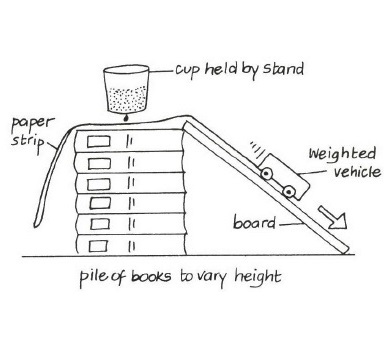
\includegraphics[width=0.45\textwidth]{./img/vso/ticker-timer.jpg}
\end{center}

\begin{description*}
%\item[Subtopic:]{}
\item[Materials:]{Long, thin strips of paper, pile of books, board, ruler}
%\item[Setup:]{}
\item[Procedure:]{Pile the books to make slopes of different heights. Attach the ticker tape (paper) to the weighted vehicle. When the vehicle is released, pull out the string in the timer cup. Repeat for a variety of heights and angles of the slope and for different weights in the vehicle.}
%\item[Hazards:]{}
\item[Questions:]{Calculate the velocity and acceleration of the vehicle using the distances between dots on the ticker timer and the average time between drops for the timing cup.}
\item[Observations:]{When the car is moving at constant speed, the dots are in regular intervals. When the car is accelerating, the distance between consecutive dots increases.}
\item[Theory:]{Velocity = distance $\div$ time. Acceleration = velocity $\div$ time. By measuring the distance between two dots over a set interval of time, both velocity and acceleration may be calculated.}
%\item[Applications:]{}
%\item[Notes:]{}
\end{description*}

\columnbreak

\subsection{Determining Acceleration Due to Gravity} \index{Acceleration! of gravity|see{Practicals}} \index{Practicals! simple pendulum} \index{Gravity! determining acceleration of|see{Practicals}} \index{Pendulum! simple|textbf}
\textbf{*NECTA PRACTICAL*}

\begin{center}
\includegraphics[width=0.4\textwidth]{./img/source/pendulum-gravity.png}
\end{center}

\begin{description*}
%\item[Subtopic:]{}
\item[Materials:]{String, stone, stopwatch, metre rule}
%\item[Setup:]{}
\item[Procedure:]{Tie the string around a stone and hang from a table. Pull the pendulum to one side and release while starting the stopwatch. Record the time taken to complete 10 full oscillations (back and forth). Record the result. Adjust the string length and repeat.}
%\item[Hazards:]{}
\item[Questions:]{Calculate the acceleration due to gravity.}
%\item[Observations:]{}
\item[Theory:]{The period $T$ of a pendulum is given by $T = 2\pi\sqrt{\cfrac{l}{g}}$, where $l$ is the length of the pendulum and $g$ the acceleration due to gravity. Solving for $g$, we see that $g = \cfrac{4\pi^2l}{T^2}$. Thus, we can calculate the acceleration due to gravity by measuring the string length and \emph{average} period (divide total time by number of periods, in this case 10).}
%\item[Applications:]{}
\item[Notes:]{The mass of the pendulum has no effect on its period.}
\end{description*}






\end{multicols}

\pagebreak